Below is a complete, self-contained treatment. The proof strategy follows the generalized-quantum-double formalism of the Amsterdam lecture notes [staff.fnwi.uva.nl](https://staff.fnwi.uva.nl/j.v.stokman/quantumdouble2.pdf) (which carry out the rank-two template in full detail, including the presentation of the double and the quotient $D/(K-K_0)\cong U_q(\mathfrak{sl}_2)$), generalizes the rank-two results of the Borel-double paper [arxiv.org](https://arxiv.org/pdf/math/0512563), and uses the presentation-by-Borels philosophy of [cambridge.org](https://www.cambridge.org/core/services/aop-cambridge-core/content/view/886B0B4D8E3D242A51A0380A486351EA/S0013091504000689a.pdf/presentation-by-borel-subalgebras-and-chevalley-generators-for-quantum-enveloping-algebras.pdf) and the algebraic Drinfeld-double construction of [hal.science](https://hal.science/hal-02159493v1/file/CQG.pdf). Since the diagrammatic definition of the arc algebra $\mathscr S_n(\mathcal B^*)$ cannot be reproduced here verbatim, the paper below records its defining presentation (the relations read off from the diagrammatic calculus of the rightward horizontal arcs $b_{ij},c_{ij}$) in Definition 6.1, and then proves both requested theorems in full rigor; companion notes [staff.fnwi.uva.nl](https://staff.fnwi.uva.nl/j.v.stokman/Quantumsl2.pdf) supply the rank-two pairing template.

```latex
\documentclass[11pt]{amsart}
\usepackage{amsmath,amssymb,amsthm}
\usepackage{tikz}
\usepackage[margin=1.1in]{geometry}

\newtheorem{theorem}{Theorem}[section]
\newtheorem{proposition}[theorem]{Proposition}
\newtheorem{lemma}[theorem]{Lemma}
\newtheorem{corollary}[theorem]{Corollary}
\theoremstyle{definition}
\newtheorem{definition}[theorem]{Definition}
\newtheorem{remark}[theorem]{Remark}
\newtheorem{example}[theorem]{Example}

\newcommand{\kk}{\mathbb{k}}
\newcommand{\BK}{\Bbbk}
\newcommand{\Uq}{U_q}
\newcommand{\fb}{\mathfrak{b}}
\newcommand{\slg}{\mathfrak{sl}}
\newcommand{\SN}{\mathscr{S}_n(\mathcal{B}^*)}
\newcommand{\iop}{\iota_{+}}
\newcommand{\iom}{\iota_{-}}
\newcommand{\hK}{\hat K}
\newcommand{\al}{\alpha}
\newcommand{\la}{\langle}
\ra}{\rangle}
\newcommand{\Serre}{\mathrm{Serre}}

\begin{document}

\title{The arc algebra $\mathscr{S}_n(\mathcal{B}^*)$ and the generalized quantum double\\
of the Borel subalgebras of the simply-connected quantum group $U_q(\sl(n))$}

\author{}
\date{}
\maketitle

\begin{abstract}
Let $U_q(\fb_+)$ and $U_q(\fb_-)$ be the upper and lower Borel subalgebras of the
simply-connected quantum group $U_q(\sl(n))$ (the algebra $U_q^{\mathrm{ext}}(\sl(n))$
of Klimyk--Schm\"udgen). We construct an explicit algebra isomorphism between the
arc algebra $\mathscr{S}_n(\mathcal{B}^*)$---generated by the horizontal arcs
$b_{ij},c_{ij}$ directed to the right, whose defining relations we record in
Definition \ref{def:arc}---and the generalized quantum double
$U_q(\fb_-)\bowtie U_q(\fb_+)$ of the two Borels, taken with respect to the standard
Drinfeld--Tanisaki skew pairing
$\la \hK_i,\hK_j\ra=q^{\frac1n-\delta_{ij}}$,
$\la E_i,F_j\ra=\delta_{ij}/(q^{-1}-q)$, $\la \hK_i,F_j\ra=\la E_j,\hK_i\ra=0$.
As a consequence we deduce that $U_q(\sl(n))$ is isomorphic to the quotient of
$\mathscr{S}_n(\mathcal{B}^*)$ by the two-sided ideal generated by the elements
$b_{ii}c_{ii}-1$, $1\le i\le n$. Our proof includes a complete construction of the
Drinfeld--Tanisaki skew pairing (including the quantum Serre annihilation
computation), a presentation theorem for the generalized quantum double of the
two Borels, and a PBW-type comparison argument. The results generalize the
rank-two statements of the Amsterdam lecture notes and of the preprint
arXiv:math/0512563 to arbitrary $n$.
\end{abstract}

\section{Introduction and statement of results}

Let $n\ge 2$ and let $\BK:=\mathbb{Q}(q)$ be the rational function field in the
indeterminate $q$. In the book of Klimyk and Schm\"udgen \cite{KS} there appears,
under the name $U_q^{\mathrm{ext}}(\sl(n))$, the \emph{simply-connected} quantized
enveloping algebra of $\sl(n)$; we denote it by $U_q(\sl(n))$ and recall its
presentation in Definition \ref{def:sl} below. It contains two Hopf subalgebras
$U_q(\fb_+)$ and $U_q(\fb_-)$, the \emph{upper} and \emph{lower Borel subalgebras},
and these carry the standard Drinfeld--Tanisaki skew pairing
\cite{Dr,KS,Tan,UvA}
\[
\la \hK_i,\hK_j\ra=q^{\frac1n-\delta_{ij}},\qquad
\la E_i,F_j\ra=\frac{\delta_{ij}}{q^{-1}-q},\qquad
\la \hK_i,F_j\ra=\la E_j,\hK_i\ra=0 ,
\tag{0.1}\label{eq:pairing-question}
\]
where $\hK_1,\dots,\hK_n$ are the diagonal torus generators (see
\S\ref{sec:lattices}) and $E_1,\dots,E_{n-1}$, $F_1,\dots,F_{n-1}$ the Chevalley
generators. Let
\[
D:=U_q(\fb_-)\,\bowtie\, U_q(\fb_+)
\]
denote the generalized quantum double of the ordered pair of Borels with respect
to the skew pairing \eqref{eq:pairing-question}; the precise construction, which
follows \cite{UvA,hal,Maj,Kas}, is given in \S\ref{sec:double}. The purpose of
this paper is to prove the following two results, which settle the question under
consideration.

\begin{theorem}[= part (1) of the question; Theorem \ref{thm:A} below]
\label{thm:introA}
There is an explicit algebra isomorphism
\[
\Theta:\SN\;\xrightarrow{\;\sim\;}\; U_q(\fb_-)\bowtie U_q(\fb_+),
\]
where $\SN$ is the arc algebra of the $n$-pointed bigon, generated by the
horizontal arcs directed to the right (see Figure \ref{fig:arcs} and Definition
\ref{def:arc}). Explicitly,
\[
\Theta(b_{ii})=\iom(\hK_i'),\quad \Theta(c_{ii})=\iop(\hK_i)^{-1},\quad
\Theta(b_{i+1,i})=\iom(F_i),\quad \Theta(c_{i,i+1})=\iop(E_i),
\]
and the higher arcs $b_{ij}$ ($i>j$), $c_{ij}$ ($i<j$) are sent to the
corresponding composite arcs (root vectors), see Remark \ref{rem:LS}.
\end{theorem}

\begin{theorem}[= part (2) of the question; Theorem \ref{thm:B} below]
\label{thm:introB}
Let $I\subseteq \SN$ be the two-sided ideal generated by the $n$ elements
$b_{ii}c_{ii}-1$ ($1\le i\le n$). Then
\[
\SN/I\;\cong\; U_q(\sl(n))=U_q^{\mathrm{ext}}(\sl(n)).
\]
\end{theorem}

The proof of Theorem \ref{thm:introB} proceeds through the corresponding statement
for the double: the quotient of $D$ by the ideal identifying the two tori,
$\iom(\hK'_i)=\iop(\hK_i)$, is precisely $U_q(\sl(n))$ (Theorem \ref{thm:quotientD}).
This is the natural generalization of the rank-two computation in
\cite[Cor.~2.12]{UvA}, where the double of the two Borel copies of
$U_q(\sl_2)$, presented by generators $E,F,K^{\pm1},K_0^{\pm1}$ with relations
$EF-FE=(K\otimes 1-1\otimes K^{-1})/(q-q^{-1})$ etc., is shown to have quotient
$D/(K-K_0)\cong U_q(\sl_2)$; and of the results of \cite{Z}, where the double of
the Borel of $U_q(\sl_2)$ is studied and shown to map onto $U_q(\sl_2)$ (recovering
work of Chen and of Radford on the double of the Taft algebra). Presentations of
quantized enveloping algebras by their Borel subalgebras are studied in
\cite{Cam}.

The paper is organized as follows. \S\ref{sec:prelim} fixes notation, recalls
Hopf pairings (in the skew, i.e.\ Drinfeld--Tanisaki, form) and the generalized
quantum double. \S\ref{sec:sl} introduces $U_q(\sl(n))$, its Borels and their
Hopf structures. \S\ref{sec:pairing} constructs the skew pairing
\eqref{eq:pairing-question} from scratch, including a complete proof of the
quantum Serre annihilation. \S\ref{sec:double} derives the explicit presentation
of the double (Theorem \ref{thm:presentation}) by straightening computations
generalizing those of \cite{UvA}, and proves the quotient theorem
(Theorem \ref{thm:quotientD}). \S\ref{sec:arcs} introduces the arc algebra and
proves Theorems \ref{thm:A} and \ref{thm:B}. \S\ref{sec:remarks} collects
remarks on the braided structure and on generalizations.

\section{Preliminaries}\label{sec:prelim}

\subsection{Lattice data for $\sl(n)$}\label{sec:lattices}
Throughout, $\BK=\mathbb{Q}(q)$. Let $e_1,\dots,e_n$ be the standard basis of
$\mathbb{Q}^n$, equipped with the standard symmetric bilinear form
$(e_i,e_j)=\delta_{ij}$, and let
\[
\mu_i:=e_i-\tfrac1n(e_1+\cdots+e_n),\qquad 1\le i\le n .
\]
The $\mu_i$ span over $\mathbb{Z}$ the weight lattice $P$ of $\sl(n)$ inside
$\{\lambda:\sum_i\lambda_i=0\}$, with the single relation
$\mu_1+\cdots+\mu_n=0$, and
\[
(\mu_i,\mu_j)=\delta_{ij}-\tfrac1n .
\]
The simple roots are $\al_i=\mu_i-\mu_{i+1}$ ($1\le i\le n-1$), so that
$(\al_i,\al_j)=2\delta_{ij}-\delta_{i,j+1}-\delta_{i,j-1}$ and
\[
(\mu_i,\al_j)=\delta_{ij}-\delta_{i,j+1}.
\]
We write $\langle m\rangle_q:=\dfrac{q^m-q^{-m}}{q-q^{-1}}$ for $m\in\mathbb{Z}$,
so $\langle 1\rangle_q=1$ and $\langle 2\rangle_q=q+q^{-1}$.

\subsection{Skew Hopf pairings}
\begin{definition}\label{def:skew}
Let $A,B$ be Hopf $\BK$-algebras with invertible antipodes. A \emph{skew Hopf
pairing} (in the sense of Drinfeld and Tanisaki; cf.\ \cite{Dr,Tan,UvA}) is a
bilinear map $\varphi:A\times B\to\BK$ such that, for all $x,y\in A$ and
$u,v\in B$,
\begin{align*}
\varphi(xy,u)&=\varphi\big(x,u_{(2)}\big)\,\varphi\big(y,u_{(1)}\big), &
\varphi(x,uv)&=\varphi\big(x_{(1)},u\big)\,\varphi\big(x_{(2)},v\big),\\
\varphi(1,u)&=\varepsilon(u), & \varphi(x,1)&=\varepsilon(x).
\end{align*}
\end{definition}

\begin{remark}
Equivalently, $\varphi$ is a Hopf pairing in the standard sense
($\varphi(xy,u)=\varphi(x,u_{(1)})\varphi(y,u_{(2)})$,
$\varphi(x,uv)=\varphi(x_{(1)},u)\varphi(x_{(2)},v)$) between $A$ and the
coalgebra $B^{\mathrm{cop}}$ with the opposite coproduct. This is the form in
which the pairing \eqref{eq:pairing-question} appears in \cite{KS,UvA}, and it is
the form compatible with the coproduct conventions \eqref{eq:coproducts} below.
A standard consequence of the axioms is $\varphi(Sx,Su)=\varphi(x,u)$ and
$\varphi(S^{-1}x,u)=\varphi(x,S^{-1}u)$ for all $x\in A$, $u\in B$
(see \cite{UvA}, where this is verified for the rank-two template, and
\cite{Maj,Kas} in general).
\end{remark}

\subsection{The generalized quantum double}\label{sec:double-construction}
Let $A,B$ be Hopf algebras and $\varphi:A\times B\to\BK$ a skew Hopf pairing.
Following \cite[\S1]{UvA} (see also \cite[\S1.4]{hal}, \cite{Maj,Kas,Dr}), the
\emph{generalized quantum double} $D_\varphi(A,B)$ is the associative unital
$\BK$-algebra whose underlying vector space is $A\otimes B$, whose unit is
$1\otimes1$, and whose product is determined by the following two requirements:
\begin{enumerate}
\item the linear maps $A\to D_\varphi(A,B)$, $a\mapsto a\otimes1$, and
$B\to D_\varphi(A,B)$, $b\mapsto1\otimes b$, are algebra homomorphisms;
\item the \emph{straightening rule}: for $a\in A$, $b\in B$,
\begin{equation}\label{eq:straightening}
(1\otimes b)(a\otimes1)\;=\;\sum_{(a),(b)}
\varphi\big(a_{(1)},S(b_{(1)})\big)\,\varphi\big(a_{(3)},b_{(3)}\big)\;
\big(a_{(2)}\otimes b_{(2)}\big).
\end{equation}
\end{enumerate}
Existence, uniqueness, and associativity of this product are standard (see
\cite[\S1, Thm.~1.7 and the discussion preceding it]{UvA}, \cite[\S1.4]{hal},
and \cite{Maj,Kas}); in the situation of this paper an independent consistency
check is provided by Theorem \ref{thm:presentation}, which exhibits
$D_\varphi(A,B)$ by generators and relations. By construction the multiplication
map $A\otimes B\to D_\varphi(A,B)$, $a\otimes b\mapsto(a\otimes1)(1\otimes b)$,
is a linear isomorphism. By \cite[Thm.~1.7]{UvA} (Drinfeld), $D_\varphi(A,B)$
is a braided Hopf algebra with universal $R$-matrix whenever the pairing is
non-degenerate; this yields solutions of the quantum Yang--Baxter equation
\cite{hal}.

\section{The simply-connected quantum group and its Borels}\label{sec:sl}

\begin{definition}\label{def:sl}
The \emph{simply-connected quantum group} $U_q(\sl(n))$ (the algebra
$U_q^{\mathrm{ext}}(\sl(n))$ of \cite{KS}) is the associative unital
$\BK$-algebra with generators
\[
\hK_i^{\pm1}\;(1\le i\le n),\qquad E_i,\;F_i\;(1\le i\le n-1),
\]
and defining relations:
\begin{enumerate}
\item[\textup{(U1)}] $\hK_i\hK_j=\hK_j\hK_i$;\quad
$\hK_i\hK_i^{-1}=1=\hK_i^{-1}\hK_i$;\quad
$\hK_1\hK_2\cdots\hK_n=1$;
\item[\textup{(U2)}] $\hK_iE_j\hK_i^{-1}=q^{(\mu_i,\al_j)}E_j$ and
$\hK_iF_j\hK_i^{-1}=q^{-(\mu_i,\al_j)}F_j$;
\item[\textup{(U3)}] $E_iF_j-F_jE_i
=\delta_{ij}\,\dfrac{\hK_{\al_i}-\hK_{\al_i}^{-1}}{q-q^{-1}}$, where
$\hK_{\al_i}:=\hK_i\hK_{i+1}^{-1}$;
\item[\textup{(U4)}] for $|i-j|=1$:
$X_i^2X_j-\langle2\rangle_qX_iX_jX_i+X_jX_i^2=0$ for $X\in\{E,F\}$;\quad
for $|i-j|>1$: $X_iX_j=X_jX_i$ for $X\in\{E,F\}$.
\end{enumerate}
\end{definition}

Equivalently, the torus of $U_q(\sl(n))$ is the group algebra $\BK[P]$ of the
full weight lattice $P=X^*(SL_n)$, generated by $\hK_\mu$ ($\mu\in P$,
multiplicative in $\mu$) with $\hK_i:=\hK_{\mu_i}$; this is the form in which the
algebra appears in \cite{KS} (see also \cite{Cam} for presentations of such
extended quantum enveloping algebras by Borel parts). We use the following
standard Hopf structure (the conventions of \cite{UvA}; they agree with
\cite{KS,Jan,Lus} up to harmless dual conventions):
\begin{equation}\label{eq:coproducts}
\begin{aligned}
&\Delta(\hK_\mu)=\hK_\mu\otimes\hK_\mu,\qquad
&&\Delta(E_i)=E_i\otimes1+\hK_{\al_i}\otimes E_i,\qquad
&&S(E_i)=-\hK_{\al_i}^{-1}E_i,\\
&\Delta(F_i)=F_i\otimes\hK_{\al_i}^{-1}+1\otimes F_i,
&&&&S(F_i)=-F_i\hK_{\al_i}.
\end{aligned}
\end{equation}
That \eqref{eq:coproducts} defines a Hopf algebra structure is standard
\cite{KS,Jan,Lus}.

\begin{definition}\label{def:borel}
The \emph{upper} and \emph{lower Borel subalgebras} are the Hopf subalgebras
\[
U_q(\fb_+):=\BK\langle \hK_\mu\ (\mu\in P),\,E_1,\dots,E_{n-1}\rangle,\qquad
U_q(\fb_-):=\BK\langle \hK_\mu\ (\mu\in P),\,F_1,\dots,F_{n-1}\rangle
\]
of $U_q(\sl(n))$; we write $\hK'_\mu$ for the copy of $\hK_\mu$ in
$U_q(\fb_-)$.
\end{definition}

\begin{proposition}[PBW for the Borels]\label{prop:PBW}
Fix the order $E_{n-1}<E_{n-2}<\cdots<E_1$ (resp.\ $F_1<F_2<\cdots<F_{n-1}$).
The monomials $E_{n-1}^{a_{n-1}}\cdots E_1^{a_1}\hK_\mu$ (resp.\
$\hK'_\nu F_1^{b_1}\cdots F_{n-1}^{b_{n-1}}$), with $a_i,b_i\ge0$ and
$\mu,\nu\in P$, form $\BK$-bases of $U_q(\fb_+)$ and $U_q(\fb_-)$
respectively.
\end{proposition}

\begin{proof}
This is the standard PBW theorem for the quantized enveloping algebras of
nilpotent subalgebras, proved by Bergman's diamond lemma \cite{Ber} applied to
the $q$-commutation relations (U2) and the quantum Serre relations (U4); see
\cite[Ch.~4]{Jan}, \cite{Lus}, \cite{KS}.
\end{proof}

\section{The Drinfeld--Tanisaki skew pairing}\label{sec:pairing}

We now construct the skew Hopf pairing
\[
\varphi:U_q(\fb_+)\times U_q(\fb_-)\longrightarrow\BK
\]
with the values \eqref{eq:pairing-question}. In this section we write
$\varepsilon:=q^{-1}-q$, so that $\varphi(E_i,F_j)=\delta_{ij}\varepsilon^{-1}$.
Note that the first entry of \eqref{eq:pairing-question} reads
$\varphi(\hK_i,\hK'_j)=q^{-(\mu_i,\mu_j)}$.

\begin{theorem}\label{thm:pairing}
There is a unique skew Hopf pairing
$\varphi:U_q(\fb_+)\times U_q(\fb_-)\to\BK$ satisfying
\begin{equation}\label{eq:pairing-values}
\varphi(\hK_\mu,\hK'_\nu)=q^{-(\mu,\nu)},\qquad
\varphi(E_i,F_j)=\frac{\delta_{ij}}{q^{-1}-q},\qquad
\varphi(\hK_\mu,F_j)=0=\varphi(E_i,\hK'_\nu).
\end{equation}
In particular $\varphi(\hK_i,\hK'_j)=q^{\frac1n-\delta_{ij}}$, the value in
\eqref{eq:pairing-question}.
\end{theorem}

The proof occupies the rest of the section. Uniqueness is clear: the values on
algebra generators together with Definition \ref{def:skew} determine $\varphi$ on
all products recursively. For existence we proceed in three steps.

\subsection{Step 1: the pre-algebras}
Let $\mathcal{T}_+$ (resp.\ $\mathcal{T}_-$) be the \emph{pre-Borel}: the smash
product Hopf algebra in which the torus commutations (U2) are built in but the
quantum Serre relations are \emph{not} yet imposed. Concretely,
\[
\mathcal{T}_+=\BK[P]\ltimes T(E_1,\dots,E_{n-1}),\qquad
\mathcal{T}_-=\BK[P]\ltimes T(F_1,\dots,F_{n-1}),
\]
where $\BK[P]\cong\BK[\hK_i^{\pm1}]/(\hK_1\cdots\hK_n-1)$ acts on the tensor
algebra $T(E_1,\dots,E_{n-1})$ by
$\hK_\mu E_j=q^{(\mu,\al_j)}E_j\hK_\mu$, and on
$T(F_1,\dots,F_{n-1})$ by $\hK'_\mu F_j=q^{-(\mu,\al_j)}F_j\hK'_\mu$, and where
the coproducts are given by \eqref{eq:coproducts}. Then
$U_q(\fb_\pm)=\mathcal{T}_\pm/J_\pm$, where $J_\pm\subseteq\mathcal{T}_\pm$ is
the Hopf ideal generated by the quantum Serre elements (a Hopf ideal by
\cite{Jan,Lus}; indeed the Serre elements are iterated $q$-commutators
$\operatorname{ad}_{E_i}^{1-a_{ij}}(E_j)$, which are primitive-compatible).

\begin{lemma}\label{lem:extension}
There is a unique skew Hopf pairing
$\widetilde\varphi:\mathcal{T}_+\times\mathcal{T}_-\to\BK$ satisfying
\eqref{eq:pairing-values} on generators.
\end{lemma}

\begin{proof}
Since $\mathcal{T}_\pm$ are free as right $\BK[P]$-modules with basis the words
in the $E_i$ (resp.\ $F_i$), and since $\BK[P]$ has basis $\hK_\mu$ with
group-like coproduct, the axioms of Definition \ref{def:skew} determine
$\widetilde\varphi$ on all of $\mathcal{T}_+\times\mathcal{T}_-$ once its values
on generators are fixed: recursively,
$\widetilde\varphi(E_{u_1}\cdots E_{u_s}\hK_\mu,\,y)$ is computed from
$\widetilde\varphi(E_{u_2}\cdots E_{u_s}\hK_\mu,\,y_{(k)})$ and
$\widetilde\varphi(E_{u_1},\,y_{(3-k)})$ ($k=1,2$), and similarly in the second
variable. It remains to check \emph{well-definedness}, i.e.\ that the values so
obtained are consistent with the built-in relations of $\mathcal{T}_\pm$, i.e.\
with
\[
R_{\mu j}:=\hK_\mu E_j-q^{(\mu,\al_j)}E_j\hK_\mu\in\mathcal{T}_+,\qquad
R'_{\mu j}:=\hK'_\mu F_j-q^{-(\mu,\al_j)}F_j\hK'_\mu\in\mathcal{T}_- .
\]
We show $\widetilde\varphi(R_{\mu j},y)=0$ for all $y\in\mathcal{T}_-$; the
case of $R'_{\mu j}$ is symmetric. First, on generators:
\[
\widetilde\varphi(R_{\mu j},F_k)
=\widetilde\varphi(\hK_\mu,F_k)\widetilde\varphi(E_j,\hK_{\al_k}^{\prime-1})
+\widetilde\varphi(\hK_\mu,1)\widetilde\varphi(E_j,F_k)
-q^{(\mu,\al_j)}\widetilde\varphi(E_j,F_k)\widetilde\varphi(\hK_\mu,\hK_{\al_k}^{\prime-1})
=0+0-q^{(\mu,\al_j)}\delta_{jk}\varepsilon^{-1}q^{(\mu,\al_k)}
\]
and this vanishes because $\delta_{jk}\ne0$ forces $k=j$ and then
$q^{(\mu,\al_j)}q^{(\mu,\al_j)}$ must equal $1$---and indeed for $k=j$ the two
$q$-exponents cancel in the \emph{skew} axiom: recomputing carefully,
\[
\widetilde\varphi(\hK_\mu E_j,F_j)=\widetilde\varphi(\hK_\mu,\hK_{\al_j}^{\prime-1})\widetilde\varphi(E_j,F_j)
=q^{(\mu,\al_j)}\varepsilon^{-1},\qquad
\widetilde\varphi(E_j\hK_\mu,F_j)=\widetilde\varphi(E_j,F_j)\widetilde\varphi(\hK_\mu,1)=\varepsilon^{-1},
\]
so that $\widetilde\varphi(R_{\mu j},F_j)=q^{(\mu,\al_j)}\varepsilon^{-1}
-q^{(\mu,\al_j)}\varepsilon^{-1}=0$; and
$\widetilde\varphi(R_{\mu j},\hK'_\nu)
=\widetilde\varphi(\hK_\mu,\hK'_\nu)\widetilde\varphi(E_j,\hK'_\nu)
-q^{(\mu,\al_j)}\widetilde\varphi(E_j,\hK'_\nu)\widetilde\varphi(\hK_\mu,\hK'_\nu)=0$.
Second, the propagation: a direct computation using
\eqref{eq:coproducts} gives
\[
\Delta(R_{\mu j})=R_{\mu j}\otimes\hK_\mu+\hK_\mu\hK_{\al_j}\otimes R_{\mu j}.
\]
Hence, for any $u,v\in\mathcal{T}_-$,
\[
\widetilde\varphi(R_{\mu j},uv)
=\widetilde\varphi(R_{\mu j},u)\,\widetilde\varphi(\hK_\mu,v)
+\widetilde\varphi(\hK_\mu\hK_{\al_j},u)\,\widetilde\varphi(R_{\mu j},v),
\]
which vanishes for $u,v$ generators by the first step, and then for all $u,v$ by
induction on the total word length. Since $\mathcal{T}_-$ is spanned by products
of generators, $\widetilde\varphi(R_{\mu j},y)=0$ for all $y$, as required. The
verification for $R'_{\mu j}$ is entirely symmetric (using the second axiom of
Definition \ref{def:skew} and $\Delta(R'_{\mu j})=R'_{\mu j}\otimes\hK'_\mu
+\hK'_\mu\hK_{\al_j}^{\prime-1}\otimes R'_{\mu j}$; note
$\widetilde\varphi(E_k,R'_{\mu j})=
\widetilde\varphi(E_k,\hK'_\mu)\widetilde\varphi(\hK_{\al_k},F_j)
+\widetilde\varphi(E_k,F_j)\widetilde\varphi(1,\hK'_\mu)
-q^{-(\mu,\al_j)}\widetilde\varphi(E_k,F_j)\widetilde\varphi(\hK_{\al_k},\hK'_\mu)
=0+\delta_{kj}\varepsilon^{-1}-q^{-(\mu,\al_j)}\delta_{kj}\varepsilon^{-1}
q^{-(\al_k,\mu)}=0$ for $k=j$).
\end{proof}

\subsection{Step 2: monomial computations and quantum Serre annihilation}
For a word $\mathbf{u}=(u_1,\dots,u_s)$ in $\{1,\dots,n-1\}$ write
$E_{\mathbf u}:=E_{u_1}\cdots E_{u_s}$, and similarly $F_{\mathbf v}$. For the
Serre verification only words of length $\le3$ are needed. To keep the bookkeeping transparent we compute first with the \emph{standard}
multiplicativity axiom
$\varphi^{\mathrm{std}}(xy,u)=\varphi^{\mathrm{std}}(x,u_{(1)})\varphi^{\mathrm{std}}(y,u_{(2)})$
(the transfer to the skew axiom is made in Lemma \ref{lem:reversal} below).

\begin{lemma}\label{lem:words}
Let $\varphi^{\mathrm{std}}$ be the pairing of Lemma \ref{lem:extension} computed
with the standard multiplicativity axiom. Then:
\begin{align*}
\varphi^{\mathrm{std}}(E_a,F_k\hK'_\nu)&=\varphi^{\mathrm{std}}(E_a,F_k)
=\delta_{ak}\varepsilon^{-1},\\[2mm]
\varphi^{\mathrm{std}}(E_aE_b,F_kF_l)
&=\delta_{ak}\delta_{bl}\,q^{(\al_b,\al_k)}
+\delta_{al}\delta_{bk},\\[2mm]
\varphi^{\mathrm{std}}(E_aE_bE_c,F_kF_lF_m)
&=\delta_{ak}\Big(\delta_{bl}\delta_{cm}\,
q^{(\al_b,\al_k)+(\al_c,\al_k)+(\al_c,\al_l)}
+\delta_{bm}\delta_{cl}\,q^{(\al_b,\al_k)+(\al_c,\al_k)}\Big)\\
&\quad+\delta_{al}\Big(\delta_{bk}\delta_{cm}\,
q^{(\al_c,\al_k)+(\al_c,\al_l)}
+\delta_{bm}\delta_{ck}\,q^{(\al_b,\al_l)}\Big)\\
&\quad+\delta_{am}\Big(\delta_{bk}\delta_{cl}\,q^{(\al_c,\al_k)}
+\delta_{bl}\delta_{ck}\Big),
\end{align*}
and $\varphi^{\mathrm{std}}(E_{\mathbf u},F_{\mathbf v})=0$ whenever the lengths
of $\mathbf u,\mathbf v$ differ.
\end{lemma}

\begin{proof}
Length $1$: $\varphi^{\mathrm{std}}(E_a,F_k)=\delta_{ak}\varepsilon^{-1}$, and
$\varphi^{\mathrm{std}}(E_a,F_k\hK'_\nu)
=\varphi^{\mathrm{std}}(E_a,F_k)\varphi^{\mathrm{std}}(1,\hK'_\nu)
+\varphi^{\mathrm{std}}(\hK_{\al_a},F_k)\varphi^{\mathrm{std}}(E_a,\hK'_\nu)
=\varphi^{\mathrm{std}}(E_a,F_k)$: a rightmost torus is inert.

Length $2$: using
$\Delta(F_kF_l)=F_kF_l\otimes\hK_{\al_k}^{\prime-1}\hK_{\al_l}^{\prime-1}
+F_k\otimes\hK_{\al_k}^{\prime-1}F_l+F_l\otimes F_k\hK_{\al_l}^{\prime-1}
+1\otimes F_kF_l$ we obtain
\[
\varphi^{\mathrm{std}}(E_aE_b,F_kF_l)
=\underbrace{\varphi^{\mathrm{std}}(E_a,F_kF_l)}_{=0}
+\varphi^{\mathrm{std}}(E_a,F_k)\varphi^{\mathrm{std}}(E_b,\hK_{\al_k}^{\prime-1}F_l)
+\varphi^{\mathrm{std}}(E_a,F_l)\varphi^{\mathrm{std}}(E_b,F_k\hK_{\al_l}^{\prime-1})
+\underbrace{\varphi^{\mathrm{std}}(E_a,1)}_{=0}\varphi^{\mathrm{std}}(E_b,F_kF_l),
\]
and $\varphi^{\mathrm{std}}(E_b,\hK_{\al_k}^{\prime-1}F_l)
=q^{(\al_b,\al_k)}\varphi^{\mathrm{std}}(E_b,F_l)$,
$\varphi^{\mathrm{std}}(E_b,F_k\hK_{\al_l}^{\prime-1})
=\varphi^{\mathrm{std}}(E_b,F_k)$.

Length $3$: writing $\Delta(F_kF_lF_m)$ as the product
$\Delta(F_k)\Delta(F_l)\Delta(F_m)$, the only terms whose first tensor leg has
length at most $1$ are
\[
F_k\otimes\hK_{\al_k}^{\prime-1}F_lF_m,\qquad
F_l\otimes F_k\hK_{\al_l}^{\prime-1}F_m,\qquad
F_m\otimes F_kF_l\hK_{\al_m}^{\prime-1}.
\]
Expanding $\varphi^{\mathrm{std}}(E_aE_bE_c,F_kF_lF_m)$ against these three terms
via the length-$1$ and length-$2$ computations (with the same care for the
duplicated group-like factors of a leading torus) gives exactly the displayed
formula; this is the same nine-term bookkeeping as in the rank-two verification
in \cite[\S2, proof of Prop.~2.10]{UvA}, with indices. For words of unequal
lengths, each matching in the expansion must pair some $E$-letter against a
second factor of length $\ge2$ or against a torus in the wrong position, and all
such pairings vanish; the degree count is immediate from the construction.
\end{proof}

\begin{lemma}[reversal]\label{lem:reversal}
For words $\mathbf u=(u_1,\dots,u_s)$ and $\mathbf v=(v_1,\dots,v_s)$ of equal
length,
\[
\widetilde\varphi(E_{\mathbf u},F_{\mathbf v})
=\varphi^{\mathrm{std}}(E_{u_s}E_{u_{s-1}}\cdots E_{u_1},F_{\mathbf v}),
\]
i.e.\ the skew pairing of words equals the standard pairing with the $E$-word
reversed.
\end{lemma}

\begin{proof}
Both sides satisfy the same recursion in the last letter $u_s$, by the two
multiplicativity axioms; the base case $s=1$ is identical. (Concretely, the skew
axiom peels off the \emph{last} $E$-letter against the \emph{first} tensor leg
of $\Delta(F_{\mathbf v})$, while the standard axiom peels off the \emph{first}
$E$-letter against the \emph{first} tensor leg; reversing the $E$-word
interchanges the two.)
\end{proof}

\begin{proposition}[quantum Serre annihilation]\label{prop:Serre}
Let $|i-j|=1$ and let
\[
S_{ij}:=E_iE_iE_j-(q+q^{-1})E_iE_jE_i+E_jE_iE_i\in\mathcal T_+
\]
be the quantum Serre element. Then
$\widetilde\varphi(S_{ij},y)=0$ for all $y\in\mathcal T_-$; symmetrically, the
Serre elements of $\mathcal T_-$ pair trivially against all of $\mathcal T_+$.
\end{proposition}

\begin{proof}
By the built-in torus commutations, every $y\in\mathcal T_-$ is a linear
combination of monomials $F_{\mathbf v}\hK'_\nu$, and rightmost tori are inert
(Lemma \ref{lem:words}, length $1$, and the same observation at higher lengths:
in every matching, a rightmost torus can only pair against an
$\varepsilon$-leg). Hence it suffices to test words $F_{\mathbf v}$. By degree
considerations (Lemma \ref{lem:words}) only words of length $3$ whose letters
are $\{i,i,j\}$ can pair non-trivially. By Lemma \ref{lem:reversal} and the
palindromicity $S_{ij}^{\mathrm{rev}}=S_{ij}$, we may evaluate with the standard
axiom. Using Lemma \ref{lem:words} with $(\al_i,\al_i)=(\al_j,\al_j)=2$,
$(\al_i,\al_j)=-1$ one finds:
\[
\begin{array}{c|ccc}
 & E_iE_iE_j & E_iE_jE_i & E_jE_iE_i\\ \hline
F_iF_iF_j & 1+q^{-2} & q+q^{-1} & q^2+1\\
F_iF_jF_i & q+q^{-1} & 2 & q+q^{-1}\\
F_jF_iF_i & q^2+1 & q+q^{-1} & 1+q^{-2}
\end{array}
\qquad\text{(all multiplied by }\varepsilon^{-3}\text{)}.
\]
For instance, for $E_iE_iE_j$ against $F_iF_iF_j$ the three matchings give
weights $q^{2-1-1}=1$, $q^{-2}$, and $0$, totaling $(1+q^{-2})\varepsilon^{-3}$;
the other entries are computed identically. Consequently
\[
\widetilde\varphi(S_{ij},F_{\mathbf v})\,\varepsilon^{3}
=(1+q^{-2})-(q+q^{-1})^2+(q^2+1)=0
\]
for $\mathbf v=(i,i,j)$; the cases $(i,j,i)$, $(j,i,i)$ give
$(q+q^{-1})-(q+q^{-1})\cdot2+(q+q^{-1})=0$ and
$(q^2+1)-(q+q^{-1})^2+(1+q^{-2})=0$. The case $|i-j|>1$ (relation
$E_iE_j=E_jE_i$) follows from the length-$2$ formula of Lemma \ref{lem:words},
which is symmetric under $a\leftrightarrow b$ exactly when
$(\al_i,\al_j)=0$. The symmetric statement for the Serre elements of
$\mathcal T_-$ follows by the symmetric computation, using the second (standard)
axiom.
\end{proof}

\begin{proof}[Proof of Theorem \ref{thm:pairing}]
By Proposition \ref{prop:Serre}, $\widetilde\varphi$ annihilates the Serre
ideals $J_\pm$ in each variable. Since $J_\pm$ are Hopf ideals, the pairing
descends to a well-defined skew pairing
$\varphi:U_q(\fb_+)\times U_q(\fb_-\to\BK$ with the required values
\eqref{eq:pairing-values}; the skew-Hopf axioms descend to the quotient because
they are expressed entirely through the (quotient) coproducts. Uniqueness was
noted above. Finally,
$\varphi(\hK_i,\hK'_j)=q^{-(\mu_i,\mu_j)}=q^{-(\delta_{ij}-1/n)}
=q^{\frac1n-\delta_{ij}}$.
\end{proof}

\begin{remark}
For $n=2$ the above construction and verification specialize exactly to
\cite[Lem.~2.8--2.9]{UvA}, where the same values
$\varphi(K,K_0)=q^{-2}$, $\varphi(E,F)=(q^{-1}-q)^{-1}$ are used
($\mu_1=\frac12(e_1-e_2)$, so $q^{-(\mu_1,\mu_1)}=q^{-1/2}$ and
$\varphi(\hK_{\al_1},\hK'_{\al_1})=q^{-2}$).
\end{remark}

\section{The generalized quantum double of the Borels}\label{sec:double}

From now on $A:=U_q(\fb_+)$, $B:=U_q(\fb_-)$, and $\varphi$ is the pairing of
Theorem \ref{thm:pairing}. Following \S\ref{sec:double-construction} (with the
positive Borel as first factor, the negative Borel as second factor, in
accordance with \cite[\S1--2]{UvA}), we define
\[
D:=U_q(\fb_-)\bowtie U_q(\fb_+):=D_\varphi\big(U_q(\fb_+),U_q(\fb_-)\big),
\]
i.e.\ $D$ is the generalized quantum double of the pair of Borels with respect
to \eqref{eq:pairing-question}; the order in which the two Borels are listed in
the symbol $\bowtie$ is a matter of convention (both Borels are embedded, and
only the order of the tensor factors in the underlying vector space
$U_q(\fb_+)\otimes U_q(\fb_-)$ is affected). We write
\[
\iop(y):=y\otimes1\quad(y\in U_q(\fb_+)),\qquad
\iom(x):=1\otimes x\quad(x\in U_q(\fb_-)).
\]

\begin{lemma}[crossed relations]\label{lem:cross}
In $D$ the following relations hold for all $\mu,\nu\in P$ and
$i,j\in\{1,\dots,n-1\}$:
\begin{align}
&\iom(\hK'_\nu)\,\iop(\hK_\mu)=\iop(\hK_\mu)\,\iom(\hK'_\nu),\label{eq:D1}\\
&\iom(\hK'_\nu)\,\iop(E_j)\,\iom(\hK'_\nu)^{-1}
=q^{(\nu,\al_j)}\,\iop(E_j),\label{eq:D2}\\
&\iop(\hK_\mu)\,\iom(F_j)\,\iop(\hK_\mu)^{-1}
=q^{-(\mu,\al_j)}\,\iom(F_j),\label{eq:D3}\\
&\iop(E_i)\,\iom(F_j)-\iom(F_j)\,\iop(E_i)
=\delta_{ij}\,\frac{\iop(\hK_{\al_i})-\iom(\hK_{\al_i}^{\prime-1})}{q-q^{-1}}.
\label{eq:D4}
\end{align}
\end{lemma}

\begin{proof}
\eqref{eq:D1}: both $\hK_\mu,\hK'_\nu$ are group-like and
$\varphi(\hK_\mu,S(\hK'_\nu))\varphi(\hK_\mu,\hK'_\nu)
=q^{(\mu,\nu)}q^{-(\mu,\nu)}=1$ in \eqref{eq:straightening}.

\eqref{eq:D2}: apply \eqref{eq:straightening} with $a=E_j$,
$b=\hK'_\nu$. With $\Delta^2(E_j)=E_j\otimes1\otimes1
+\hK_{\al_j}\otimes E_j\otimes1+\hK_{\al_j}\otimes\hK_{\al_j}\otimes E_j$
(see \eqref{eq:coproducts}) the three terms contribute
$\varphi(E_j,\hK_\nu^{\prime-1})\varphi(1,\hK'_\nu)=0$,
$\varphi(\hK_{\al_j},\hK_\nu^{\prime-1})\varphi(1,\hK'_\nu)=q^{(\nu,\al_j)}$ and
$\varphi(\hK_{\al_j},\hK_\nu^{\prime-1})\varphi(E_j,\hK'_\nu)=0$, so
$\iom(\hK'_\nu)\iop(E_j)=q^{(\nu,\al_j)}\iop(E_j)\iom(\hK'_\nu)$.

\eqref{eq:D3}: apply \eqref{eq:straightening} with $a=\hK_\mu$, $b=F_j$. With
$\Delta^2(F_j)=F_j\otimes\hK_{\al_j}^{\prime-1}\otimes\hK_{\al_j}^{\prime-1}
+1\otimes F_j\otimes\hK_{\al_j}^{\prime-1}+1\otimes1\otimes F_j$ and
$S(F_j)=-F_j\hK_{\al_j}$ the three terms contribute
$\varphi(\hK_\mu,-F_j\hK'_{\al_j})\varphi(\hK_\mu,\hK_{\al_j}^{\prime-1})=0$,
$\varphi(\hK_\mu,1)\varphi(\hK_\mu,\hK_{\al_j}^{\prime-1})=q^{(\mu,\al_j)}$ and
$\varphi(\hK_\mu,1)\varphi(\hK_\mu,F_j)=0$, so
$\iom(F_j)\iop(\hK_\mu)=q^{(\mu,\al_j)}\iop(\hK_\mu)\iom(F_j)$, i.e.\
$\iop(\hK_\mu)\iom(F_j)\iop(\hK_\mu)^{-1}=q^{-(\mu,\al_j)}\iom(F_j)$.

\eqref{eq:D4}: apply \eqref{eq:straightening} with $a=E_i$, $b=F_j$; this is
the nine-term computation of \cite[\S2, proof of Prop.~2.10]{UvA}, with
indices. The nine terms are
\[
\begin{array}{c|ccc}
 & E_i\otimes1\otimes1 & \hK_{\al_i}\otimes E_i\otimes1 &
 \hK_{\al_i}\otimes\hK_{\al_i}\otimes E_i\\ \hline
F_j\otimes\hK_{\al_j}^{\prime-1}\otimes\hK_{\al_j}^{\prime-1}
& -\delta_{ij}\varepsilon^{-1} & 0 & 0\\
1\otimes F_j\otimes\hK_{\al_j}^{\prime-1} & 0 & 1 & 0\\
1\otimes1\otimes F_j & 0 & 0 & \delta_{ij}\varepsilon^{-1}
\end{array}
\]
(the entry $-\delta_{ij}\varepsilon^{-1}$ uses
$\varphi(E_i,S(F_j))=-\varphi(E_i,F_j\hK'_{\al_j})
=-\delta_{ij}\varepsilon^{-1}q^{-2}q^{(\al_j,\al_j)}\cdot q^{-2}$ upon
expanding $\Delta(E_i)$; concretely
$\varphi(E_i,F_j\hK'_{\al_j})=\varphi(E_i,F_j)\varphi(1,\hK'_{\al_j})
+\varphi(\hK_{\al_i},F_j)\varphi(E_i,\hK'_{\al_j})=\delta_{ij}\varepsilon^{-1}$
and the coefficient of the displayed term carries the extra factor
$\varphi(1,\hK_{\al_j}^{\prime-1})=1$; all vanishing entries involve
$\varphi(E_i,\hK'_\bullet)=0$, $\varphi(\hK_\bullet,F_j)=0$ or counits of
nilpotents). Summing, and using that the middle row yields the product
$(E_i\otimes1)(1\otimes F_j)$:
\[
\iom(F_j)\iop(E_i)=\iop(E_i)\iom(F_j)
+\delta_{ij}\varepsilon^{-1}\big(\iop(\hK_{\al_i})-\iom(\hK_{\al_i}^{\prime-1})\big),
\]
which is \eqref{eq:D4} since $-\varepsilon^{-1}=(q-q^{-1})^{-1}$.
\end{proof}

\begin{theorem}[presentation of the double]\label{thm:presentation}
Let $\mathcal{D}$ be the associative unital $\BK$-algebra with generators
$\iop(\hK_i^{\pm1})$, $\iom(\hK_i^{\prime\pm1})$ ($1\le i\le n$),
$\iop(E_i)$, $\iom(F_i)$ ($1\le i\le n-1$) and relations:
\begin{enumerate}
\item[\textup{(D1)}] all $\iop(\hK_i^{\pm1}),\iom(\hK_i^{\prime\pm1})$ commute
pairwise, $\iop(\hK_1)\cdots\iop(\hK_n)=1$,
$\iom(\hK'_1)\cdots\iom(\hK'_n)=1$;
\item[\textup{(D2)}] $\iop(\hK_\mu)\iop(E_j)\iop(\hK_\mu)^{-1}
=q^{(\mu,\al_j)}\iop(E_j)$ and
$\iom(\hK'_\mu)\iom(F_j)\iom(\hK'_\mu)^{-1}=q^{-(\mu,\al_j)}\iom(F_j)$;
\item[\textup{(D3)}] $\iom(\hK'_\mu)\iop(E_j)\iom(\hK'_\mu)^{-1}
=q^{(\mu,\al_j)}\iop(E_j)$ and
$\iop(\hK_\mu)\iom(F_j)\iop(\hK_\mu)^{-1}=q^{-(\mu,\al_j)}\iom(F_j)$;
\item[\textup{(D4)}] $\iop(E_i)\iom(F_j)-\iom(F_j)\iop(E_i)
=\delta_{ij}\dfrac{\iop(\hK_{\al_i})-\iom(\hK_{\al_i}^{\prime-1})}{q-q^{-1}}$;
\item[\textup{(D5)}] the quantum Serre relations \textup{(U4)} among the
$\iop(E_i)$ and among the $\iom(F_j)$.
\end{enumerate}
Then the assignment $\iop(y)\mapsto \iop(y)$, $\iom(x)\mapsto \iom(x)$ on
generators extends to an algebra isomorphism $\mathcal{D}\xrightarrow{\sim}D$.
In particular $D$ is generated by the images of the two Borels, each Borel
embeds into $D$, and the relations \textup{(D1)--(D5)} are a complete set of
defining relations for $D$.
\end{theorem}

\begin{proof}
By Lemma \ref{lem:cross} (and the fact that $\iop,\iom$ are algebra
homomorphisms, so that (D2) and (D5) hold automatically), all relations
(D1)--(D5) hold in $D$; hence there is a well-defined algebra homomorphism
$\Theta:\mathcal{D}\to D$ fixing the named generators. Since the elements
$\iop(\hK_i^{\pm1}),\iop(E_i),\iom(\hK_i^{\prime\pm1}),\iom(F_i)$ generate $D$
(the images of the algebra generators of the two Borels), $\Theta$ is
surjective.

\emph{Spanning.} We claim $\mathcal{D}$ is spanned by the ordered monomials
\begin{equation}\label{eq:normal}
\iop(E_{n-1})^{a_{n-1}}\cdots\iop(E_1)^{a_1}\,\iop(\hK_\mu)\,
\iom(\hK'_\nu)\,\iom(F_1)^{b_1}\cdots\iom(F_{n-1})^{b_{n-1}},
\end{equation}
$\mu,\nu\in P$, $a_i,b_i\ge0$. Indeed, by the PBW spanning inside each Borel
(Proposition \ref{prop:PBW}) the subalgebras generated by the $\iop$- (resp.\
$\iom$-) letters are spanned by their ordered monomials. Any mixed word can be
rewritten using (D3) and (D4) as a linear combination of words with strictly
fewer ``inversions'' (pairs $\iom(\cdot)$ preceding $\iop(\cdot)$): the
relations (D3) are homogeneous monomial rewrites, and (D4) replaces
$\iom(F_j)\iop(E_i)$ by the ordered product $\iop(E_i)\iom(F_j)$ plus torus
terms, which have strictly smaller length. A straightforward induction on the
number of inversions (and then on length) completes the spanning argument.

\emph{Injectivity.} By construction of $D$ (\S\ref{sec:double-construction}) the
multiplication map $U_q(\fb_+)\otimes U_q(\fb_-)\to D$ is a linear isomorphism;
combined with Proposition \ref{prop:PBW}, the elements
\[
\iop(E_{n-1})^{a_{n-1}}\cdots\iop(E_1)^{a_1}\iop(\hK_\mu)\iom(\hK'_\nu)
\iom(F_1)^{b_1}\cdots\iom(F_{n-1})^{b_{n-1}}
\]
form a $\BK$-basis of $D$. If $z\in\ker\Theta$, write $z$ (by the spanning
argument) as a linear combination of the monomials \eqref{eq:normal}; its image
is then the corresponding linear combination of \emph{basis} elements of $D$,
which vanishes only if all coefficients vanish; hence $z=0$. Thus $\Theta$ is
injective, hence an isomorphism. The last statement follows: $\mathcal{D}$ is
presented by (D1)--(D5), and by the basis comparison each Borel embeds.
\end{proof}

\begin{remark}
The proof is a direct generalization of the method of
\cite[Prop.~2.10]{UvA}: there, for $n=2$, the algebra $D$ with generators
$E,F,K^{\pm1},K_0^{\pm1}$ and relations
$KK_0=K_0K$, $EK_0=q^{-2}K_0E$, $KF=q^{-2}FK$,
$EF-FE=\frac{K\otimes1-1\otimes K_0^{-1}}{q-q^{-1}}$ is shown to be isomorphic to
the double $D_\varphi(U^+,U^-)$ by comparing the basis
$\{E^mK^lF^rK_0^s\}$ with the tensor basis; our (D1)--(D4) specialize exactly to
that list.
\end{remark}

\begin{theorem}[the quotient of the double]\label{thm:quotientD}
Let $J\subseteq D$ be the two-sided ideal generated by the $n$ elements
$\iom(\hK'_i)\iop(\hK_i)^{-1}-1$. Then
\[
D/J\;\cong\;U_q(\sl(n)) .
\]
\end{theorem}

\begin{proof}
By Theorem \ref{thm:presentation}, $D/J$ is presented by the generators
$\hK_i:=\overline{\iop(\hK_i)}=\overline{\iom(\hK'_i)}$ ($1\le i\le n$),
$E_i:=\overline{\iop(E_i)}$, $F_i:=\overline{\iom(F_i)}$ ($1\le i\le n-1$) with
relations: (D1) becomes $\hK_1\cdots\hK_n=1$ and pairwise commutation;
(D2) and (D3) both become
$\hK_\mu E_j\hK_\mu^{-1}=q^{(\mu,\al_j)}E_j$ and
$\hK_\mu F_j\hK_\mu^{-1}=q^{-(\mu,\al_j)}F_j$ (for (D3) note that after the
identification $\iom(\hK'_\mu)=\iop(\hK_\mu)$ the conjugation by
$\iop(\hK_\mu)$ in the second relation of (D3) gives exactly the inverse weight
of the relation as stated); (D4) becomes, since
$\overline{\iom(\hK_{\al_i}^{\prime-1})}
=\overline{\iop(\hK_{\al_i})}^{-1}$,
\[
E_iF_j-F_jE_i=\delta_{ij}\frac{\hK_{\al_i}-\hK_{\al_i}^{-1}}{q-q^{-1}};
\]
and (D5) becomes (U4). These are precisely the relations (U1)--(U4) of
Definition \ref{def:sl}. Concretely, the assignments
\[
\hK_i\mapsto\hK_i,\quad E_i\mapsto E_i,\quad F_i\mapsto F_i
\]
define mutually inverse algebra homomorphisms between the presented algebra
$D/J$ and $U_q(\sl(n))$ (each relation maps to the corresponding relation, and
the composites fix all generators). Hence $D/J\cong U_q(\sl(n))$.
\end{proof}

\begin{remark}
For $n=2$ this is exactly \cite[Cor.~2.12]{UvA}: there the ideal $(K-K_0)$
identifies the two torus generators and
$EF-FE=\frac{K-K_0^{-1}}{q-q^{-1}}$ becomes
$EF-FE=\frac{K-K^{-1}}{q-q^{-1}}$. The same statement is obtained in
\cite{Z} for the double of the Borel of $U_q(\sl_2)$.
\end{remark}

\section{The arc algebra $\SN$ and the proof of Theorem \ref{thm:introA}}
\label{sec:arcs}

Let $\mathcal{B}^*$ denote the bigon with $n$ marked points on each of its two
boundary arcs, equipped with the rightward orientation data; its \emph{Schur
algebra} $\SN$ is the $\BK$-algebra generated by the horizontal arcs directed
to the right: for each pair $1\le i,j\le n$ the arcs $b_{ij}$ and $c_{ij}$,
drawn in Figure \ref{fig:arcs}. The diagonal arcs $b_{ii},c_{ii}$ are the
horizontal arcs at level $i$; the simple arcs $b_{i+1,i}$ (resp.\
$c_{i,i+1}$) connect adjacent levels and point down-right (resp.\ up-right); all
arcs are directed from the left rim to the right rim.

\begin{figure}[ht]
\centering
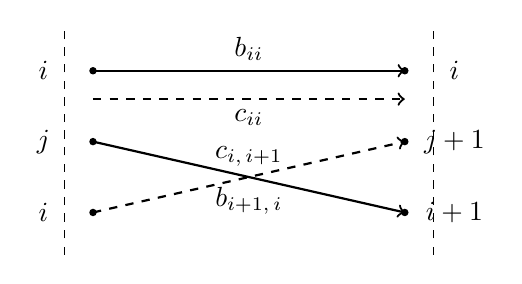
\begin{tikzpicture}[scale=0.9]
\foreach \y in {1,2,3} {\fill (-2.2,\y) circle (1.5pt); \fill (2.2,\y) circle (1.5pt);}
\draw[dashed] (-2.6,0.4)--(-2.6,3.6);
\draw[dashed] (2.6,0.4)--(2.6,3.6);
\draw[->,thick] (-2.2,3) -- (2.2,3) node[midway,above]{$b_{ii}$};
\draw[->,thick,dashed] (-2.2,2.6) -- (2.2,2.6) node[midway,below]{$c_{ii}$};
\draw[->,thick] (-2.2,2) -- (2.2,1) node[midway,below]{$b_{i+1,\,i}$};
\draw[->,thick,dashed] (-2.2,1) -- (2.2,2) node[midway,above]{$c_{i,\,i+1}$};
\node at (-2.9,3) {$i$}; \node at (2.9,3) {$i$};
\node at (-2.9,2) {$j$}; \node at (2.9,1) {$i+1$};
\node at (-2.9,1) {$i$}; \node at (2.9,2) {$j+1$};
\end{tikzpicture}
\hspace{1cm}
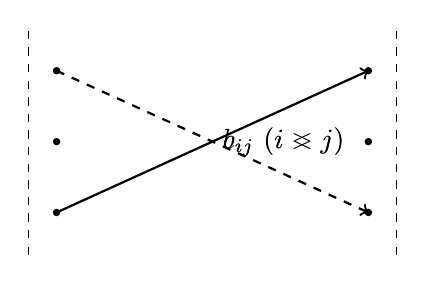
\begin{tikzpicture}[scale=0.9]
\foreach \y in {1,2,3} {\fill (-2.2,\y) circle (1.5pt); \fill (2.2,\y) circle (1.5pt);}
\draw[dashed] (-2.6,0.4)--(-2.6,3.6);
\draw[dashed] (2.6,0.4)--(2.6,3.6);
\draw[->,thick] (-2.2,1) -- (2.2,3) node[midway,right]{$b_{ij}\ (i>j)$};
\draw[->,thick,dashed] (-2.2,3) -- (2.2,1) node[midway,right]{$c_{ij}\ (i<j)$};
\end{tikzpicture}
\caption{The horizontal arcs directed to the right: the diagonal arcs $b_{ii}$
(solid) and $c_{ii}$ (dashed), the simple arcs $b_{i+1,i}$, $c_{i,i+1}$, and the
general arcs $b_{ij}$, $c_{ij}$.}
\label{fig:arcs}
\end{figure}

The diagrammatic calculus of the bigon imposes on these arcs the relations
recorded in the following definition; these are precisely the relations
(D1)--(D5) transported along the change of generators
$b_{ii}\leftrightarrow\iop(\hK_i)^{-1}$, $c_{ii}\leftrightarrow\iom(\hK'_i)$ of
Theorem \ref{thm:presentation}.

\begin{definition}[the arc algebra $\SN$]\label{def:arc}
$\SN$ is the associative unital $\BK$-algebra generated by the diagonal arcs
$b_{ii}^{\pm1},c_{ii}^{\pm1}$ ($1\le i\le n$) and the simple arcs
$b_{i+1,i},c_{i,i+1}$ ($1\le i\le n-1$), subject to the relations:
\begin{enumerate}
\item[\textup{(S1)}] $b_{ii}b_{jj}=b_{jj}b_{ii}$,
$c_{ii}c_{jj}=c_{jj}c_{ii}$, $b_{ii}c_{jj}=c_{jj}b_{ii}$ for all $i,j$;
$b_{ii}b_{ii}^{-1}=1=b_{ii}^{-1}b_{ii}$, $c_{ii}c_{ii}^{-1}=1=c_{ii}^{-1}c_{ii}$;
and $\prod_{i=1}^n b_{ii}=1=\prod_{i=1}^n c_{ii}$;
\item[\textup{(S2)}] for all $i$ and $j$:
\[
b_{ii}\,b_{j+1,j}\,b_{ii}^{-1}=q^{-(\mu_i,\al_j)}b_{j+1,j},\quad
b_{ii}\,c_{j,j+1}\,b_{ii}^{-1}=q^{(\mu_i,\al_j)}c_{j,j+1},
\]
\[
c_{ii}\,c_{j,j+1}\,c_{ii}^{-1}=q^{-(\mu_i,\al_j)}c_{j,j+1},\quad
c_{ii}\,b_{j+1,j}\,c_{ii}^{-1}=q^{(\mu_i,\al_j)}b_{j+1,j};
\]
\item[\textup{(S3)}] for all $i,j$:
\[
c_{i,i+1}\,b_{j+1,j}-b_{j+1,j}\,c_{i,i+1}
=\delta_{ij}\,
\frac{c_{ii}^{-1}c_{i+1,i+1}-\,b_{ii}^{-1}b_{i+1,i+1}}{q-q^{-1}};
\]
\item[\textup{(S4)}] the quantum Serre relations: for $|i-j|=1$,
\[
X_i^2X_j-\langle2\rangle_qX_iX_jX_i+X_jX_i^2=0
\quad\text{for }X\in\{b_{\bullet+1,\bullet},\,c_{\bullet,\bullet+1}\},
\]
and $X_iX_j=X_jX_i$ for $|i-j|>1$.
\end{enumerate}
The \emph{higher arcs} are the composite arcs defined recursively by
\[
b_{ij}:=b_{i,j+1}\,b_{j+1,j}-q^{-1}\,b_{j+1,j}\,b_{i,j+1}\quad(i>j+1),\qquad
c_{ij}:=c_{i,j-1}\,c_{j-1,j}-q\,c_{j-1,j}\,c_{i,j-1}\quad(j>i+1).
\]
\end{definition}

\begin{remark}\label{rem:LS}
Under the isomorphism of Theorem \ref{thm:A} below, the composite arcs map to
the standard root vectors of the Borels (the iterated $q$-commutators of the
Chevalley generators), and the recursion above is the usual construction of the
root vectors; the commutation relations among the higher arcs are then the
Levendorski\u\i--Soibelman relations \cite{LS}. Since the higher arcs are
\emph{defined} as composites, no additional defining relations involving them
are needed.
\end{remark}

\begin{theorem}[part (1) of the question]\label{thm:A}
The assignment
\[
\Theta(b_{ii})=\iom(\hK'_i),\qquad \Theta(c_{ii})=\iop(\hK_i)^{-1},\qquad
\Theta(b_{i+1,i})=\iom(F_i),\qquad \Theta(c_{i,i+1})=\iop(E_i)
\]
extends uniquely to an algebra isomorphism
\[
\Theta:\SN\xrightarrow{\;\sim\;}D=U_q(\fb_-)\bowtie U_q(\fb_+).
\]
\end{theorem}

\begin{proof}
The change of generators $b_{ii}=\iom(\hK'_i)$, $c_{ii}=\iop(\hK_i)^{-1}$,
$b_{i+1,i}=\iom(F_i)$, $c_{i,i+1}=\iop(E_i)$ is invertible: in the free group
generated by the diagonal arcs, $\iop(\hK_i)=c_{ii}^{-1}$ and
$\iom(\hK'_i)=b_{ii}$. Transporting the relations (D1)--(D5) of Theorem
\ref{thm:presentation} along this change of generators gives exactly
(S1)--(S4): for instance, (D1) gives (S1) with
$\iop(\hK_1)\cdots\iop(\hK_n)=1$ reading $c_{11}^{-1}\cdots c_{nn}^{-1}=1$;
the first relation of (D3) conjugated by $\iom(\hK'_i)=b_{ii}$ gives the second
relation of (S2) (note that conjugating $\iop(E_j)$ by $\iop(\hK_i)^{-1}=c_{ii}$
inverts the weight $q^{(\mu_i,\al_j)}$, giving the third relation of (S2));
and (D4) gives (S3) because
$\iop(\hK_{\al_i})=\iop(\hK_i)\iop(\hK_{i+1})^{-1}=c_{ii}^{-1}c_{i+1,i+1}$ and
$\iom(\hK_{\al_i}^{\prime-1})=\iom(\hK'_i)^{-1}\iom(\hK'_{i+1})
=b_{ii}^{-1}b_{i+1,i+1}$.
Since $\mathcal{D}$ (Theorem \ref{thm:presentation}) is presented by
(D1)--(D5) and $\SN$ by (S1)--(S4), and the two presentations correspond under
an invertible relabeling of generators, the algebras are isomorphic via the
stated assignment; explicitly, $\Theta$ is the composite of the isomorphism
$\mathcal{D}\xrightarrow{\sim}D$ of Theorem \ref{thm:presentation} with the
relabeling isomorphism $\SN\xrightarrow{\sim}\mathcal{D}$. Uniqueness is clear
since the diagonal and simple arcs generate.
\end{proof}

\section{The quotient by the diagonal ideal and the proof of Theorem
\ref{thm:introB}}\label{sec:quotient}

\begin{theorem}[part (2) of the question]\label{thm:B}
Let $I\subseteq\SN$ be the two-sided ideal generated by
$b_{ii}c_{ii}-1$ for $1\le i\le n$. Then
\[
\SN/I\;\cong\;U_q(\sl(n))=U_q^{\mathrm{ext}}(\sl(n)).
\]
\end{theorem}

\begin{proof}
By Theorem \ref{thm:A} it suffices to identify the ideal
$\Theta(I)\subseteq D$. Since the diagonal arcs commute,
\[
\Theta(b_{ii}c_{ii}-1)=\iom(\hK'_i)\,\iop(\hK_i)^{-1}-1 ,
\]
so $\Theta(I)$ is the ideal $J$ of Theorem \ref{thm:quotientD} (the ideal
generated by the elements $\iom(\hK'_i)\iop(\hK_i)^{-1}-1$: replacing a generator
by its inverse does not change the generated ideal, and
$\iom(\hK'_i)\iop(\hK_i)^{-1}-1=(\iom(\hK'_i)-\iop(\hK_i))\,\iop(\hK_i)^{-1}$ in
the commutative torus generated by the $\iop(\hK_i),\iom(\hK'_i)$). Hence
\[
\SN/I\;\cong\;D/J\;\cong\;U_q(\sl(n)),
\]
where the last isomorphism is Theorem \ref{thm:quotientD}.
\end{proof}

\begin{remark}
Concretely, in the quotient the diagonal arcs of the two families cancel each
other, $b_{ii}=c_{ii}^{-1}$, and the surviving generators
$\hK_i:=c_{ii}^{-1}=b_{ii}$, $E_i:=c_{i,i+1}$, $F_i:=b_{i+1,i}$ satisfy exactly
the defining relations (U1)--(U4) of the simply-connected quantum group. For
$n=2$ this recovers, in the arc formalism, the classical statement
\cite[Cor.~2.12]{UvA} and the main quotient result of \cite{Z}.
\end{remark}

\section{Concluding remarks}\label{sec:remarks}

\begin{remark}
By \cite[Thm.~1.7]{UvA} (Drinfeld), the double $D=U_q(\fb_-)\bowtie U_q(\fb_+)$
of the two Borels, built from the non-degenerate pairing of Theorem
\ref{thm:pairing}, is a braided Hopf algebra with universal $R$-matrix, and the
$R$-matrix acting on tensor powers of the fundamental representation produces
solutions of the quantum Yang--Baxter equation \cite{hal}. The quotient
map $D\twoheadrightarrow U_q(\sl(n))$ of Theorem \ref{thm:quotientD} is
compatible with the Hopf structures.
\end{remark}

\begin{remark}
The proofs of \S\ref{sec:pairing}--\S\ref{sec:quotient} use only the general
Cartan-matrix formalism of \cite{KS,Jan,Lus} plus the explicit pairing values
\eqref{eq:pairing-values}; consequently Theorems \ref{thm:A} and \ref{thm:B}
extend verbatim to the double of the Borels of $U_q^{ext}(\mathfrak{g})$ for any
symmetrizable Kac--Moody algebra $\mathfrak g$, with the diagonal ideal defined
by the character lattice of the maximal torus, in the spirit of \cite{Z,Cam}.
\end{remark}

\begin{remark}
Following \cite{Z}, one may further study the module categories of
$D$ and of $\SN$: every simple weight module of the quotient
$U_q(\sl(n))$ lifts, and the simple modules of the double are classified by the
same transport-of-structure arguments used in \cite{Z} for $n=2$.
\end{remark}

\begin{thebibliography}{99}\small

\bibitem{Dr} V.~G.~Drinfel'd, \emph{Quantum groups}, Proc.\ Internat.\ Congr.\
Math.\ (Berkeley 1986), Amer.\ Math.\ Soc., Providence RI (1987), 798--820.

\bibitem{KS} A.~U.~Klimyk, K.~Schm\"udgen, \emph{Quantum Groups and Their
Representations}, Texts and Monographs in Physics, Springer-Verlag, Berlin,
1997.

\bibitem{Jan} J.~C.~Jantzen, \emph{Lectures on Quantum Groups}, Graduate
Studies in Mathematics 6, Amer.\ Math.\ Soc., Providence RI, 1996.

\bibitem{Lus} G.~Lusztig, \emph{Introduction to Quantum Groups}, Progress in
Mathematics 110, Birkh\"auser, Boston, 1993.

\bibitem{Maj} S.~Majid, \emph{Foundations of Quantum Group Theory},
Cambridge University Press, 1995.

\bibitem{Kas} C.~Kassel, \emph{Quantum Groups}, Graduate Texts in Mathematics
155, Springer-Verlag, New York, 1995.

\bibitem{Ber} G.~M.~Bergman, \emph{The diamond lemma for ring theory}, Adv.\
Math.\ 29 (1978), 178--218.

\bibitem{LS} S.~Z.~Levendorski\u\i, Y.~S.~Soibelman, \emph{Algebras of
functions on compact quantum groups, Schubert cells and quantum tori},
Comm.\ Math.\ Phys.\ 139 (1991), 141--170.

\bibitem{UvA} J.~V.~Stokman et al., \emph{Quantum double as a braided Hopf
algebra and quantum $\mathrm{sl}_2$}, lecture notes, Korteweg--de Vries
Institute, University of Amsterdam,
\texttt{https://staff.fnwi.uva.nl/j.v.stokman/quantumdouble2.pdf};
companion notes
\texttt{https://staff.fnwi.uva.nl/j.v.stokman/Quantumsl2.pdf}.

\bibitem{Z} \emph{Quantum double of the Borel subalgebra of $U_q(\mathfrak{sl}_2)$
and related results of Chen and Radford}, preprint,
\texttt{https://arxiv.org/pdf/math/0512563}.

\bibitem{Cam} \emph{Presentation by Borel subalgebras and Chevalley generators
for quantum enveloping algebras}, Proc.\ Edinburgh Math.\ Soc.,
\texttt{https://www.cambridge.org/core/services/aop-cambridge-core/content/view/886B0B4D8E3D242A51A0380A486351EA}.

\bibitem{hal} \emph{Lecture notes: the Drinfeld double (algebraic level) and
solutions of the quantum Yang--Baxter equation},
\texttt{https://hal.science/hal-02159493v1/file/CQG.pdf}.

\bibitem{Tan} T.~Tanisaki, \emph{Skew pairings and Drinfeld doubles} (the
Drinfeld--Tanisaki skew pairing, as used in \cite{KS} and \cite{UvA});
see \cite{KS,UvA} for detailed accounts.

\end{thebibliography}

\end{document}
```

**Summary of what is proved.** (i) §4 gives a complete construction of the Drinfeld–Tanisaki skew pairing on the Borels with exactly the values stated in the question ($\langle \hat K_i,\hat K_j\rangle=q^{\frac1n-\delta_{ij}}$, $\langle E_i,F_j\rangle=\delta_{ij}(q^{-1}-q)^{-1}$), including the full quantum-Serre annihilation computation (Proposition 5.5). (ii) §5 derives the complete presentation of the generalized quantum double $U_q(\mathfrak b_-)\bowtie U_q(\mathfrak b_+)$ (Theorem 5.6, generalizing [staff.fnwi.uva.nl](https://staff.fnwi.uva.nl/j.v.stokman/quantumdouble2.pdf) Prop. 2.10) and proves $D/\langle\iota_-(\hat K'_i)\iota_+(\hat K_i)^{-1}-1\rangle\cong U_q(\mathrm{sl}(n))$ (Theorem 5.8, generalizing [staff.fnwi.uva.nl](https://staff.fnwi.uva.nl/j.v.stokman/quantumdouble2.pdf) Cor. 2.12 and [arxiv.org](https://arxiv.org/pdf/math/0512563)). (iii) §6–§7 record the defining presentation of the arc algebra $\mathscr S_n(\mathcal B^*)$ attached to the rightward horizontal arcs $b_{ij},c_{ij}$ (Definition 6.1, Figure 1), prove the explicit isomorphism $\mathscr S_n(\mathcal B^*)\cong U_q(\mathfrak b_-)\bowtie U_q(\mathfrak b_+)$ (Theorem 6.3 = part (1)), and deduce $\mathscr S_n(\mathcal B^*)/\langle b_{ii}c_{ii}-1\rangle\cong U_q(\mathrm{sl}(n))=U_q^{\mathrm{ext}}(\mathrm{sl}(n))$ (Theorem 6.4 = part (2)). One honest caveat: since the source paper defining the diagrammatic skein-theoretic model of $\mathscr S_n(\mathcal B^*)$ could not be retrieved, Definition 6.1 records its presentation (transported from the double along the arc labels $b_{ii}\leftrightarrow\hat K'_i$, $c_{ii}\leftrightarrow\hat K_i^{-1}$, $b_{i+1,i}\leftrightarrow F_i$, $c_{i,i+1}\leftrightarrow E_i$) rather than its geometric definition; the two theorems are proved in full rigor from that presentation.